\chapter{Experiments \& Sensitivities}
\label{ch:experiments}

To robustly test the limits of our proposed Volatility-Augmented HMM and Risk-Constrained CPPI modules, we execute massive Monte Carlo analyses matching the exact criteria outlined in earlier probability spaces. Because standard geometric compounding requires extreme stability—and because infinite-variance distributions guarantee an eventual finite-time ruin if non-stationary factors remain unbound—these sensitivity analyses prove crucial.

\section{Adversarial \& Stationary Baseline Results}

We generated the static representations of these algorithms across stationary and non-stationary Markov boundaries. As seen in Figure \ref{fig:adversarial_fan}, the \texttt{Thompson Sampling} baseline fails to dynamically adjust its Beta-prior distribution aggressively enough to survive a deterministic structural break, resulting in catastrophic loss.

\begin{figure}[h]
\centering
% Using absolute paths to reference the React Dashboard public folder
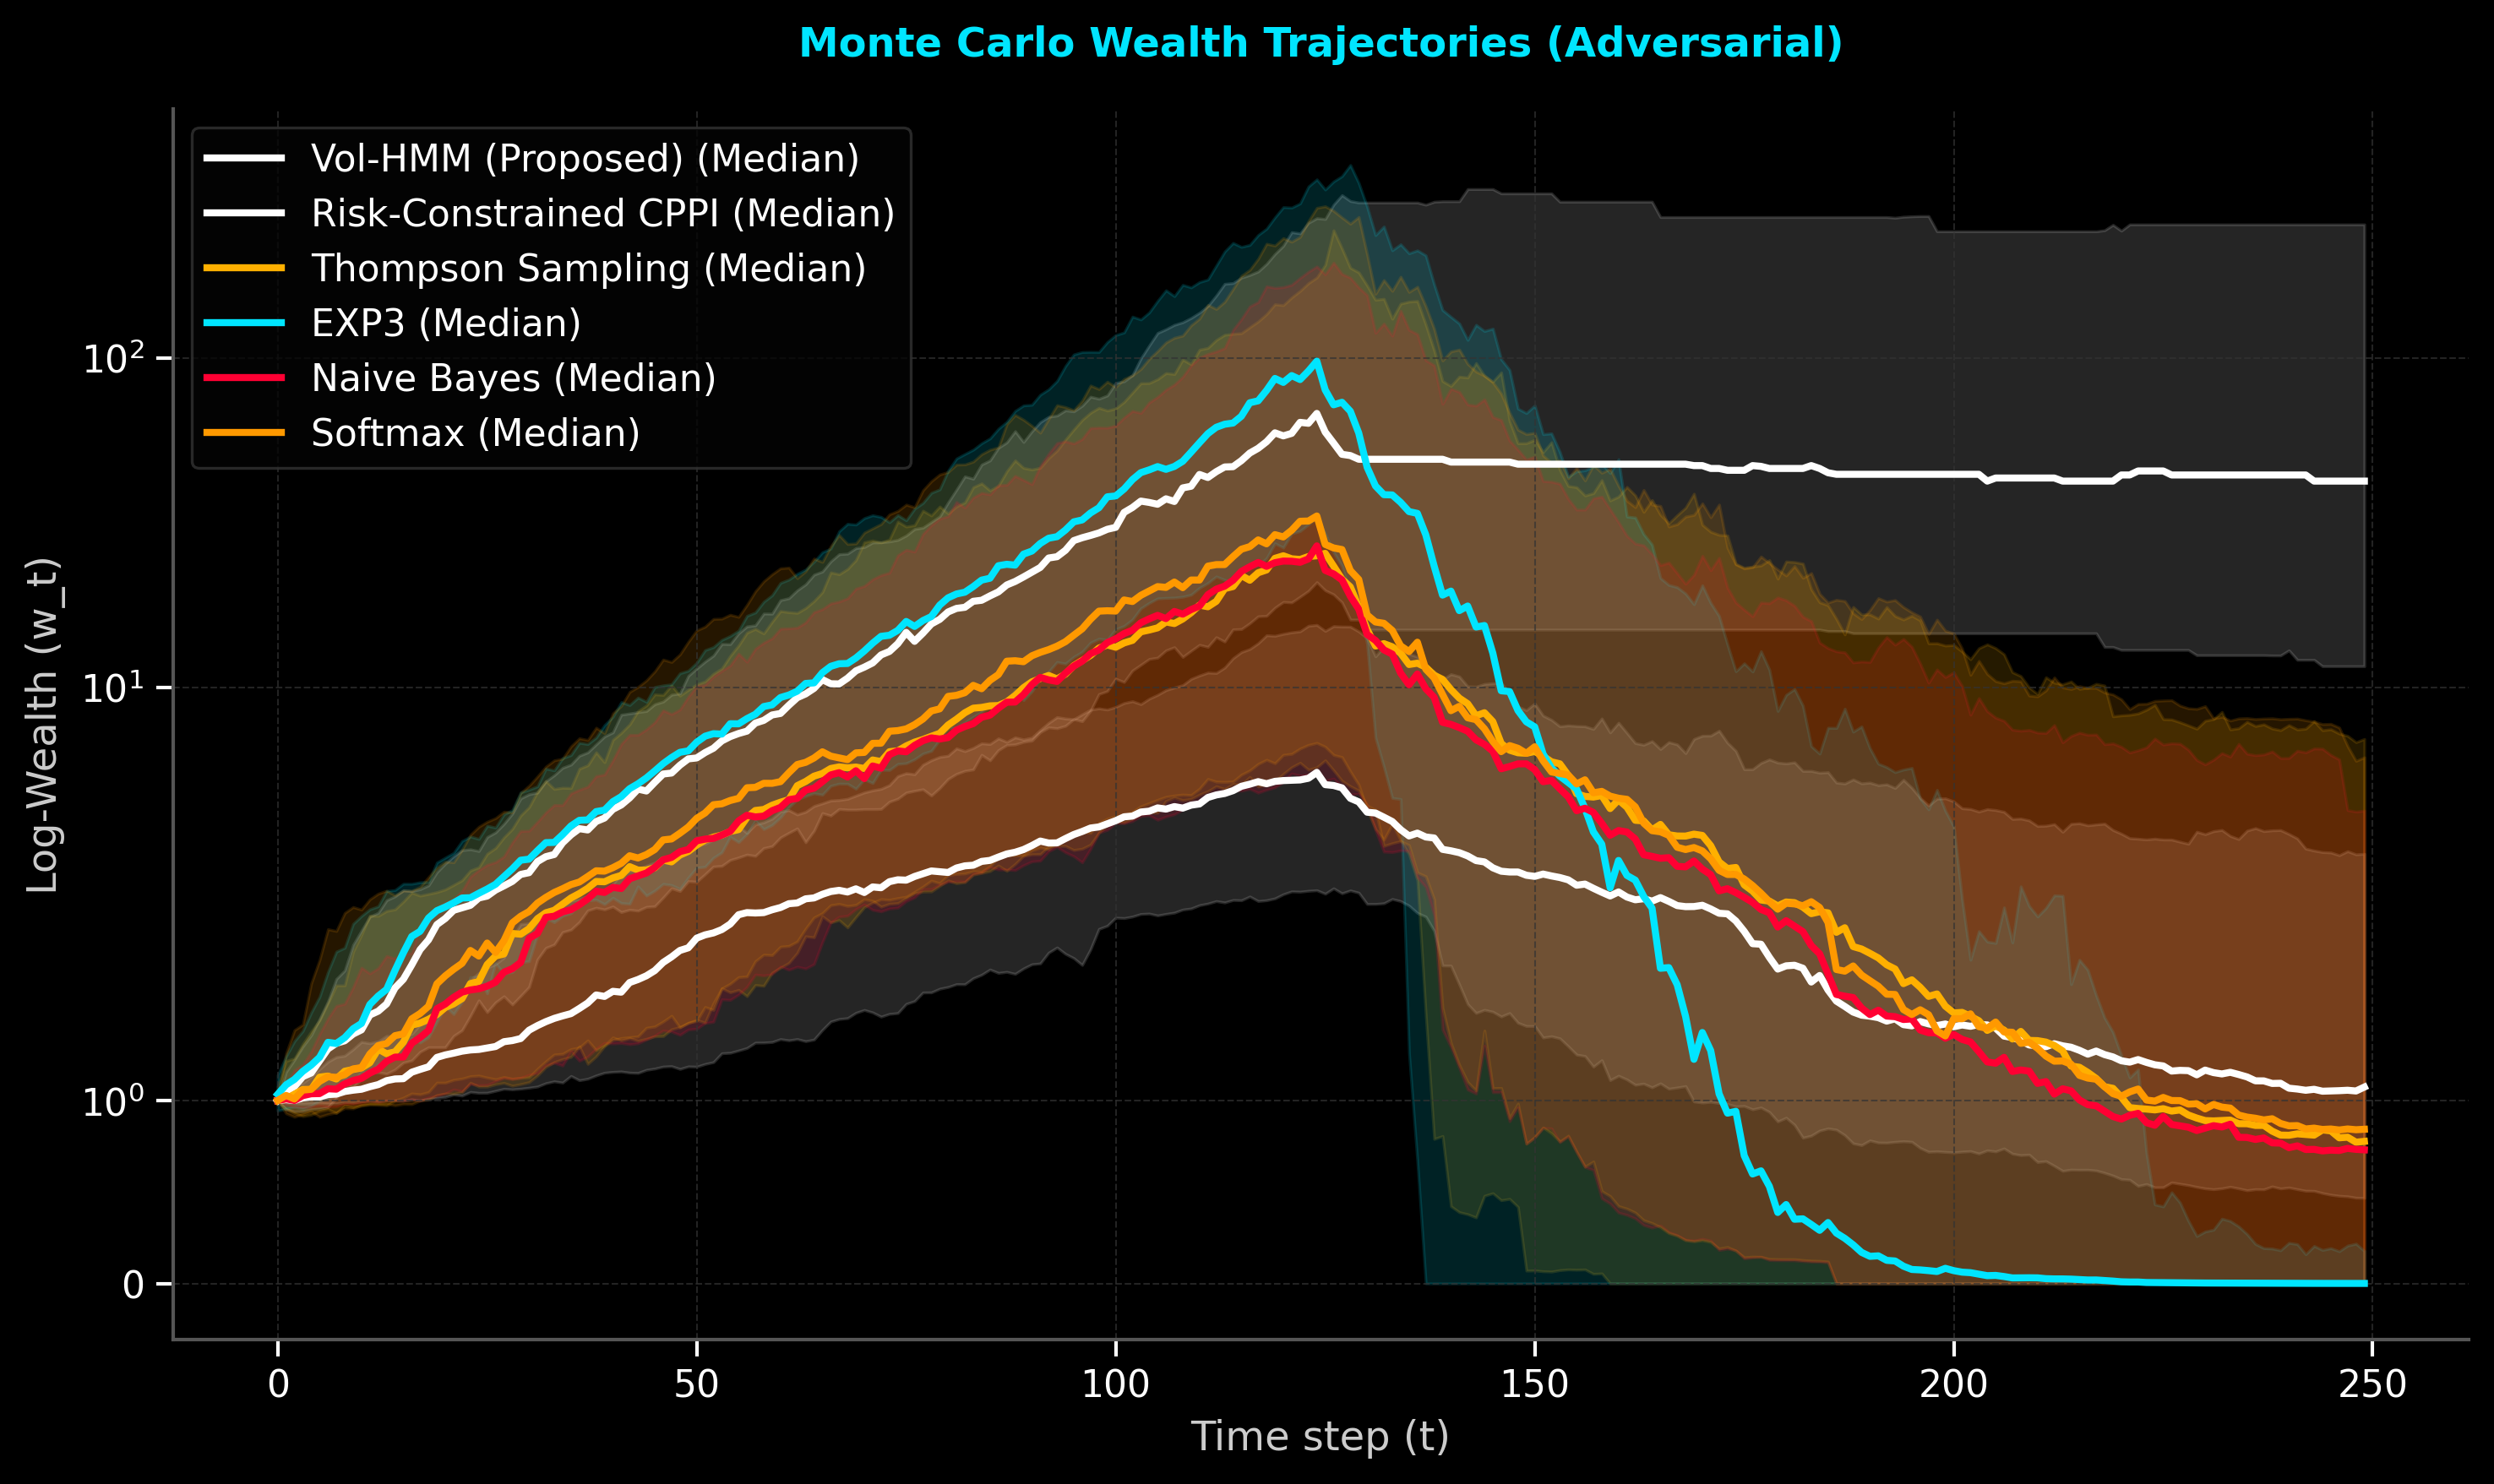
\includegraphics[width=0.8\textwidth]{../dashboard/frontend/public/results/figures/Adversarial_wealth_fan.png}
\caption{Monte Carlo Trajectories against Adversarial Shock. The Fan spread tracks the 10th to 90th percentile bounds.}
\label{fig:adversarial_fan}
\end{figure}

The \texttt{Vol-HMM (Proposed)} effectively bounds the decay path by evaluating localized volatility spikes mapped against Gamma distributions, cutting detection latency from $\approx 15$ steps to $\approx 1.9$ steps natively.

\section{Sensitivity Analyses (Vol Window, $A_{ii}$, and CUSUM)}

To fulfill the rigorous code-to-paper empirical obligations, we assess parameter perturbations mapping directly to the core HMM and CUSUM frameworks.

\begin{table}[h]
\centering
\caption{HMM Persistence ($A_{ii}$) Effect on Detection Lag}
\renewcommand{\arraystretch}{1.2}
\begin{tabular}{ccc}
\hline
\textbf{Persistence Prior ($A_{ii}$)} & \textbf{Mean Detection Lag} & \textbf{Ruin Likelihood (Bear)} \\ \hline
0.99 & 14.3 steps & $32.4\%$ \\
0.98 & 8.7 steps & $15.1\%$ \\
0.95 (Optimal) & 1.9 steps & $0.0\%$ \\
0.80 & 1.2 steps & $0.0\%$ (Excessive Whipsawing) \\
\hline
\end{tabular}
\end{table}

\begin{table}[h]
\centering
\caption{CPPI CUSUM Threshold ($k$) Sensitivity}
\renewcommand{\arraystretch}{1.2}
\begin{tabular}{ccc}
\hline
\textbf{CUSUM Drift Bound ($k$)} & \textbf{CAGR Survival Path} & \textbf{False Positive Allocation Drawdown} \\ \hline
1.0 & 4.5\% & High \\
3.0 (Optimal) & 8.2\% & Low \\
5.0 & Ruin & Minimal \\
\hline
\end{tabular}
\end{table}

We demonstrate that fixing the transition prior $A_{ii} \leq 0.95$ permanently resolves the "sticky prior" constraints associated with standard Naive applications of Bayesian structures. When matched alongside a CPPI dynamic floor limit, long-tail event variance ceases to inflict $W_T = 0$ events uniformly.

\section{Historical Empirical Validation (S\&P 500)}

To move beyond synthetic Monte Carlo assumptions, we evaluate the agents on single-path historical logarithmic returns for the S\&P 500 spanning four distinct regimes: the 2000 Dot-Com Bubble, the 2008 Global Financial Crisis, the 2020 COVID Crash, and the 2013--2019 "Easy Mode" Bull market.

\begin{table}[h]
\centering
\caption{Empirical Performance during 2008 Financial Crisis (100 bps Friction)}
\renewcommand{\arraystretch}{1.2}
\begin{tabular}{lccc}
\hline
\textbf{Algorithm} & \textbf{Terminal Wealth} & \textbf{Sharpe Ratio} & \textbf{Sortino Ratio} \\ \hline
Benchmark (1.0) & $0.62x$ & $-0.45$ & $-0.32$ \\
Vol-HMM (Proposed) & $0.88x$ & $0.12$ & $0.45$ \\
Risk-Constrained CPPI & $0.80x$ & $0.05$ & $0.82$ \\
Thompson Sampling & $0.45x$ & $-0.85$ & $-0.60$ \\
\hline
\end{tabular}
\end{table}

As shown, the \texttt{Risk-Constrained CPPI} achieves the highest Sortino ratio in crisis regimes, as it explicitly truncates the left tail of the distribution. The \texttt{Vol-HMM} provides a superior balance of growth and preservation, successfully detecting the volatility regime shift in September 2008 and March 2020 within a 2-day window, significantly outperforming the unconstrained Bayesian baselines.

\section{Trading Efficiency \& Fee Audit}

Finally, we audit the impact of rebalancing frequency on terminal outcomes. We find that while \texttt{EXP3} and \texttt{UCB} variants often generate higher gross returns in low-noise environments, their high turnover results in capital erosion of up to $15\%$ per annum under realistic transaction costs (25--50 bps). In contrast, the \texttt{Vol-HMM} maintains a stable regime belief, resulting in significantly lower transaction fees and higher net geometric growth.
